%introduction
In this section we will analyse the {\bf  main differences} between the {\bf  \textit{AXI interconnect} inside the Cortex} M3 Design Start and the {\bf \textit{CCCAXI connect}} module that {\bf we implemented}.
\newline

In particular, the {\bf first paragraph} explains how the signals pass through the two AXI and the {\bf different delays} given by them, while the {\bf second one} focuses on some {\bf gating differences} of our implementation, discussing the {\bf pros and cons}.
\newline

{\color{Blue}{\subsection{Time Differences}}}

Comparing the two implementations and the relative simulations, it is possible to notice that the handshake protocol provided by \textit{CCCAXI connect} is faster than the one of \textit{AXI interconnect}.
\newline

This difference is caused by the fact that the \textit{CCCAXI connect} is simpler and designed to run specifically in this enviroment. The \textit{AXI interconnect} must provide various features (for example customize the number of masters/slaves, the arbitration betwen masters, safety, support clock-gating, ...). The difference is conceptually due to a different approach: designing a specific IP or designing a generic one.
\newline

The timing difference is due to a different number of intermediate steps that the signal finds in its path and by the nature of those steps; infact, while in \textit{CCCAXI connect} there is simply a muxer/demuxer gating the signals, inside the \textit{AXI interconnect} there are more (and more sophisticated) steps:
\newline


{\flushleft
\begin{description}

\item[Slave Coupler:]Used as interface for the Cortex M3, it converts the \textbf{AXI3 protocol} of the processor to the \textbf{AXI4-lite protocol} of \textit{Xbar} and the peripherals. As a consequence, this conversion introduces a delay into the main signal of both write and read operations (in our implementation the conversion is provided by the component \textit{AXI4lite adapter} which hides a simple wire connection for only the signals used).

\item[Xbar:]Its main function is to initialize and manage the communication between a \textit{Slave Coupler} and a \textit{Master Coupler}. Therefore, the delay introduced by it is not only for choosing the right master interface to associate but also to achieve the handshake protocol among the interfaces (in our implementation the handshake protocol is managed by the master and slave themselves).
The Figure \ref{RWXbar} shows an example of read and write operations of the \textit{Xbar}.

\item[Master Coupler:]Like the \textit{Slave Coupler} but without conversion logic, it is used as interface for peripheral.

\end{description}
}

For more information about the \textit{AXI interconnection} and its components, see \cite{AXIInterconnectGuide}.
\newline



{\color{Blue}{\subsection{Signal Propagation}}}

An other {\bf difference} between the two considered modules can be found in the {\bf way} with which the {\bf various signals} on the bus are {\bf propagated}. In particular, the \textit{AXI interconnection} always propagates the data and address signals to all the slaves, while propagates the control signals (the ones involved into the handshake) only to the proper slave. The data read from the slave and its response in case of a write are propagated only from the right slave to the right master. On the other hand, \textit{CCCAXI connect} {\bf propagates each signal only between the interested components}, without any form of broacasting.
\newline

A {\bf pro} of our implementation could be the fact that the {\bf addresses} that came as output from the processor are {\bf kept private} and forwarded only to the proper slave: the other components are left detatched from the interaction. This can prevent the possibility from a malicious agent to sniff these sensible data if not explicitly counsulted by the current master.
An other positive fact is that our component is {\bf more compliant with the specifications}.
\newline

{\bf On} the {\bf other side}, our choiche {\bf increases the complexity of} the {\bf propagation} of addresses and data, requiring a more complex, power hungry and costly mux/demux.
Moreover, as shown in \ref{PSO}, our implementation uses {\bf lot of IOBs}, in such a number that makes it quite unrealistic to be implemented with the given architecture. %In our defence, if some one will oneday implement it, we can say "In our machine, it worked... It must be a {\bfVivado fautl!}".
\newline
However we managed to {\bf fully execute} the program loaded in the memory, {\bf without} raising {\bf any error}, as we observed by the output of the uarlite. 

\begin{figure}[!hb]
  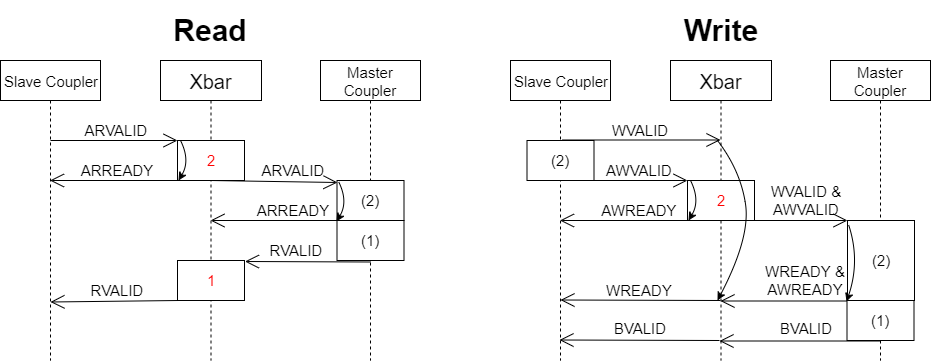
\includegraphics[width=\textwidth]{./../../img/Images/Read_Write_xbar}
  \caption{Read and write communication on Xbar with {\color{Red}Xbar delays} and other latencies (curly arrow to identify the communication's sections)}
  \label{RWXbar}
\end{figure}

\begin{figure}[!hb]
  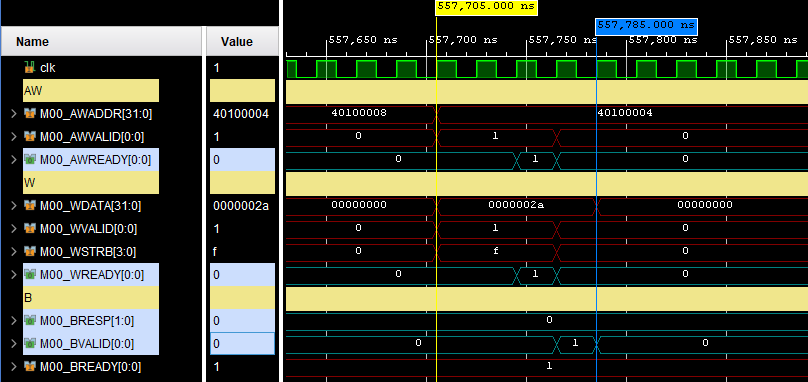
\includegraphics[width=\textwidth]{./../../img/Images/CCCAXI_waform_write}
  \caption{Write example of the CCCAXI}
  \label{WriteCCC}
\end{figure}

\begin{figure}[!hb]
  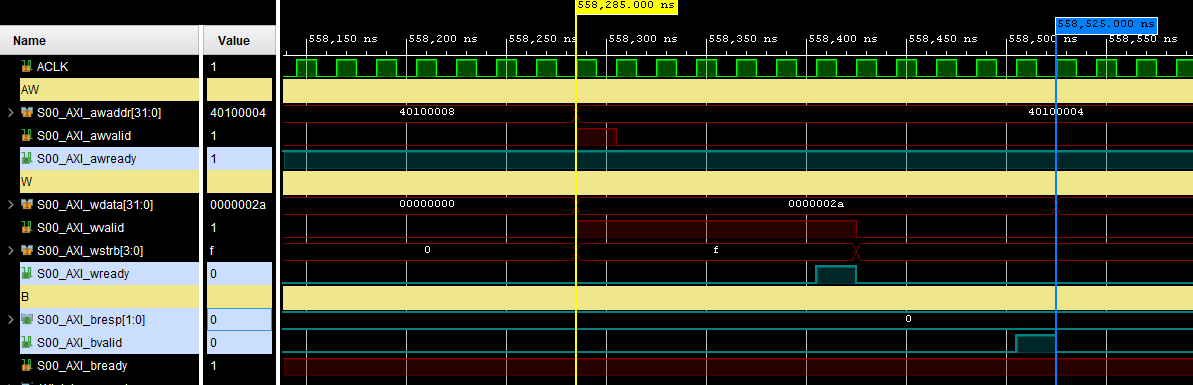
\includegraphics[width=\textwidth]{./../../img/Images/AXI_waveform_write}
  \caption{Write example of the AXI}
  \label{WriteAXI}
\end{figure}

\begin{figure}[!hb]
  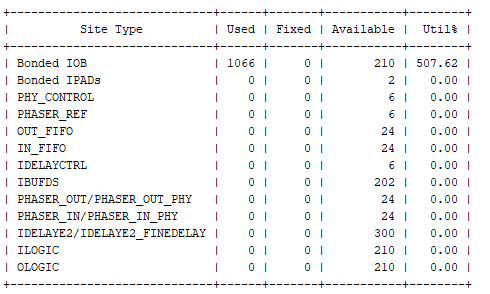
\includegraphics[width=\textwidth]{./../../img/Images/Tabella_post_synthesis}
  \caption{Post syntesis outcome}
  \label{PSO}
\end{figure}
